\documentclass[12pt]{article}
\usepackage{graphicx}
\usepackage[margin=1.0in]{geometry}
\usepackage{color, colortbl}

\definecolor{LightCyan}{rgb}{0.88,1,1}
\definecolor{LightRose}{rgb}{1,0.88,0.88}
\definecolor{LightGreen}{rgb}{0.88,1,0.88}

\title{FADC pulse compression}
\author{Gagik Gavalian}
\date{May 2017}

\begin{document}

\begin{titlepage}
\maketitle
\begin{abstract}
Bit packing algorithm for Flash Analog to Digital Converter (FADC) pulse compression
for CLAS12 experiment is investigated. The data reduction from bit packing is compared 
to standard compression routines like GZIP and LZ4. 

\end{abstract}
\end{titlepage}

\section{Introduction}

This article discusses methods to compress pulses from FADC in the data stream.
Instead of compression algorithms which are CPU intensive, a bit packing is used.
The pulse has to be transformed into series of progressive integers then packed
as four bit samples.

\section{Pulse structure}

In CLAS12 experiment the readout of detector PMT's is done using Flash ADC's which
sample the charge every 4~ns, and report 100 samples per reading. Each sampling is 
recorded into a 13 bit integer.  Currently the pulses are stored in series of 16 bit words
amounting to 200 byte arrays for each pulse. The purpose of this note is to investigate
bit packing algorithms on these pulses to determine what compression ratio can be 
achieved.

\section{Transforming the pulse}

The FADC pulse first has to be transformed into incremental integer series, where
each next number is larger than previous. The difference between each sample will
be stored in a packed array. Here are the transformation steps:

\begin{itemize}
\item subtract the minimum value of the pulse from the sample.
\item construct cumulative integral distribution.
\item construct an array with differences between the bins.
\item isolate lower 4 bits and upper 8 bits into two arrays.
\item create an array of bytes half the size of the pulse and pack 4 bit array into it.
\item write non-zero elements of 8 bit array into a smaller array using one byte per element.
\end{itemize} 

In the example of CLAS12 pulses, the data structure consists of one 2 byte word for
minimum of the pulse, followed by 50 byte array that encodes 100 4 bit integers, followed
by 1 byte with first non-zero element of the upper 8 bit array, followed by non-zero bytes
from 8 bit array. The minimum information that all pulses have in common are 52 bytes,
this is quarter of the bytes used in uncompressed pulse, followed by 10-15 (in average)
bytes of upper 8 bit array. This makes the pulse information factor of 3 smaller, than 
recording the pulse into 16 bit words (200 bytes).



\begin{figure}[!ht]
\begin{center}

 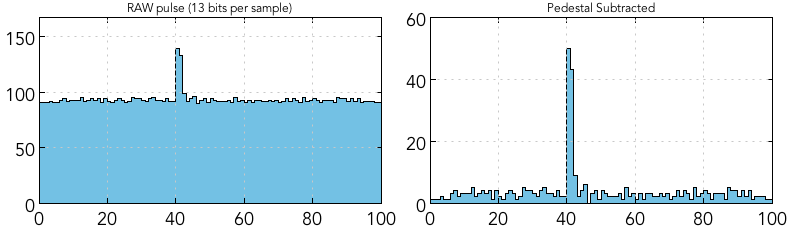
\includegraphics[width=5in]{pics/fadc_pulse_reduction.png}
 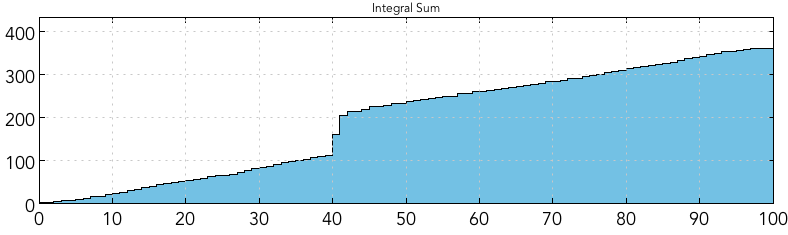
\includegraphics[width=5in]{pics/fadc_pulse_summ.png}

 \caption {Typical pulse from Electro-Magnetic Calorimeter, top left) raw pulse, top right) pedestal subtracted pulse, bottom) integral sum of the pulse.}
 \label{FADC_PULSE}
 \end{center}
\end{figure}

A typical pulse from FADC is show in Figure~\ref{FADC_PULSE}. The first two steps of
pulse transformation are shown on Figure~\ref{FADC_PULSE} a) and b). First the minimum
bin is subtracted from the pulse, leading to the figure on top right corner, then integral sum
is constructed, show on the bottom of Figure~\ref{FADC_PULSE}.

Next the integral sum is split into two arrays, first one containing low 4 bits of the
difference between neighboring bins, and high 8 bits, show on Figure~\ref{FADC_PULSE_BITS}.

\begin{figure}[!ht]
\begin{center}

 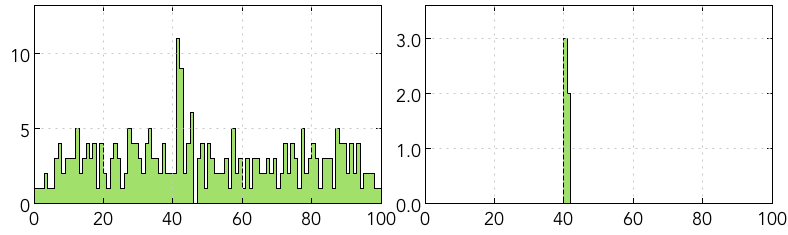
\includegraphics[width=5in]{pics/fadc_pulse_bits.png}

 \caption {Separated arrays of low (4) and high (8) bites. left) low 4 bites of difference array,
 right) high 8 bites of difference array. }
 \label{FADC_PULSE_BITS}
 \end{center}
\end{figure}

The two arrays are encoded differently. First distribution (left on Figure~\ref{FADC_PULSE_BITS}) is encoded into 50 bytes, using 4 bits for each sample (0-15), with preceding 2 bytes containing the subtracted pedestal for the pulse. The second array is written out using one byte per signal, after
throwing away leading and trailing 0s. One byte is first written for first bin with no 0 content, followed
by N samples of 8 bits until the last non zero bin is reached.

In the above given example occupied 55 bytes (instead of 200) to fully describe the pulse.
Depending on the width of the pulse in average 10-15 bytes are used to encode high bits of 
the pulse, while the low bits are always encoded using 52 bites.

\section{Benchmarks}

For our tests we used a file from Electromagnetic Calorimeter cosmic runs. We took 9372 sample
pulses and bit-packed them into compact arrays and wrote output to binary file, for further 
compression tests.

Performed test show that bit packing algorithm works well for reducing data network traffic 
from data acquisition by factor of 2/3. An initial improvement of factor of 57\% can be achieved 
also by compressing the pulse with GZIP, but compression algorithms are CPU intensive and several
threads have to be used to compress data at data acquisition level, while bit packing is not as intensive
and will reduce data by larger factor. The tests show that amount of data to be written to the tapes 
(assuming compression is applied) also improves significantly , only 2/3 of the data will be written.

\begin{table}[!h]
\begin{center}
\begin{tabular}{  p{8cm} | p{2cm} | p{1.5cm} }
\hline 
Method & File Size & Ratio \\
\hline 
\hline 
Raw & 1.87~MB & 1.00 \\
Raw (LZ4) & 0.81~MB & 0.43 \\
Raw (GZIP) & 0.71~MB & 0.37 \\
\rowcolor{LightCyan}
Bit Packed &  0.63~MB & 0.34 \\
Bit Packed (LZ4) & 0.55~MB & 0.29 \\
\rowcolor{LightRose}
Bit Packed (GZIP) & 0.48~MB & 0.26 \\
Bit Packed Lossy  & 0.39~MB & 0.21 \\
\rowcolor{LightGreen}
Bit Packed Lossy (GZIP) & 0.27~MB & 0.14 \\
\hline
\end{tabular}
\caption{Data sizes compared to raw pulse and bit packed. The samples were further
compressed using GZIP and LZ4 to present data reduction on tapes.}
\end{center}
\end{table}

\section{Conclusion}

It has been shown that bit packing algorithms can help reducing FADC pulse data during data
acquisition, initial compression ratio for pulse is 0.37, a huge improvement on data rates. It has
been demonstrated that bit packed data can be further compressed (when writing to the tapes)
by factor of 0.67 those saving tape storage in the long run. Further speed tests will be performed 
to compare this algorithm with online compression speed.

The encoding described above is completely lose-less and the pull pulse will be reconstructed 
from the data. The low (4 bits) part of the pulse is always described with 52 bytes. It is possible
to smooth the background distribution described with 4 bites to further compress by applying 
smoothing function. 


\end{document}